\documentclass[3p]{elsarticle}
\usepackage{amsmath, amsfonts, amssymb, bm, graphicx}

\title{Three dimensional cold-plasma simulations on adaptive grids with internal boundaries}

\author[sintef]{Robert Marskar}
\ead{robert.marskar@sintef.no}
\address[sintef]{SINTEF Energy Research}

\def\diff{\ensuremath{\text{d}}}
\def\bmx{\ensuremath{\bm{x}}}

\begin{document}
\begin{abstract}

\end{abstract}
\maketitle

\section{Introduction}
A streamer is a non-thermal, self-propagating weakly ionized plasma filament with a bright (i.e. radiating) head which precedes electrical sparks. A streamer moves due to the motion of non-Maxwellian electrons in the head, and may move with or against the electron drift direction. A streamer which moves \emph{with} the electron drift direction contains a net negative charge in its head, and is therefore called a negative streamer. Conversely, a streamer which moves \emph{opposite} to the electron drift direction contains a net positive charge in the head and is called a positive streamer. Generally speaking, both modes propagate due to electron impact ionization (i.e. when ionization exceeds attachment) in the streamer head. However, a positive streamer additionally requires access to free electrons in front of the head, which are normally supplied through photoionization mechanisms or electron detachment from a background ionization. In air, for example, a positive streamer propagates primarily by electron excitation of molecular nitrogen which can radiatively relax down to the ground state. Since the energy difference between the excited and ground states of nitrogen exceed the ionization potential of molecular oxygen, photo-relaxataion can produce seed electrons by photoionization of molecular oxygen. 

Streamers are abundant in nature and are relevant in a number of industries. For example, streamer modeling is relevant for the high-voltage industry since its dynamics determine the electrical withstand. Furthermore, since a streamer may initiate in a super-critical field region (i.e. field regions where the electric field is above the breakdown field) and can then propagate through a subcritical region by field self-enhancement, streamer modeling can determine the minimum background field through which a streamer can propagate. In other types of industries, streamers are actually desired. For example, in high-intensity discharge (HID) lamps, a streamer is responsible for establishing the conductive path where the initial electric arc strikes. In such applications, a streamer crossing the gas gap is warranted, but its attachment of the streamer to the glass can damage the lamp and must be prevented. 

The computational modelling of weakly ionized plasmas is inherently difficult due to the existence multiple length and time scales, as well as the presence of numerical stiffness. For atmospheric air, for example, a streamer channel is surrounded by a space charge layer with a thickness in the micrometer range, while the streamer itself can propagate tens of centimeters. Typical aspect ratios up to 1000 can therefore easily be envisioned, and adaptive mesh refinement (AMR) is almost universally required for numerically resolving such phenomena, especially in three dimensions. The inclusion of internal boundary conditions inside the computational domain leads to additional complexities, and it essential that these can be resolved in a way that remain compatible with AMR. Other difficulties of a more fundamental nature are related to the treatment of the various species (neutral, ions, electrons). For the most part, neutrals and ions are close to equilibrium for weakly ionized plasmas, and the velocity distribution function (VDF) is therefore Maxwellian so that they can be treated in the continuum (i.e. fluid) approximation. This is not necessarily the case for electrons whose VDF may be far from Maxwellian and may therefore require a kinetic (i.e. particle based) treatment. Hybrid models that combine kinetic and fluid approaches are, strictly speaking, still in their infancy but are starting to gain traction in the plasma community. The stability of such methods have been a challenge due to the inherent statistical noise that is present in e.g. Direct Monte Carlo Simulations (DMCS) or Particle-In-Cell (PIC) based approaches. Methods for direct solutions of the Boltzmann equation are also being developed. The Discrete Velocity Method, for example, reduces the Boltzmann equation to a system of hyperbolic equations for a set of velocities and is therefore a direct analogue of the Discrete Ordinates Method (DOM) for the radiative transfer equation (RTE). The DVM is, strictly speaking, different from Lattice-Boltzmann methods due to the number of velocities that are included in the discretization of phase space (usually $10^3$ for DVM versus $10^1$ for LBM). Nonetheless, simplified plasma models are still of great interest because of their simplicity and their straightforward compatibility with embedded boundary conditions. 

In this paper we examine a minimal plasma model consisting of mass balance and field equations. We include embedded boundaries in the form of electrodes and dielectrics, and examine the interaction of streamers with such surfaces. 

The structure of this paper is as follows: In Sec.~\ref{sec:theory} we review the minimal plasma model. We outline our numerical methods in Sec.~\ref{sec:method} and provide numerical examples in Sec.~\ref{sec:examples}. Some remarks regarding the minimal streamer model are given in Sec.~\ref{sec:remarks}. 

\section{Theory}
\label{sec:theory}
The minimal plasma model consists of charge (or mass) conservation for the massive species (i.e. electrons, ions, and neutral molecules), the Poisson equation for the electric field, radiative transfer equations for photon transport, and a scalar conservation equation for the charge-balance on dielectric surfaces. 

\subsection{Electrodynamic equations}
\label{subsec:electrodynamic}
For a weakly ionized plasma such as a streamer, the streamer current is sufficiently small so that one may safely disregard magnetic field effects. The remaining equation for the evolution of the electromagnetic field is Poisson's equation:
\begin{equation}
  \nabla\cdot\left(\epsilon\nabla\Phi\right) = -\frac{\rho}{\epsilon_0},
\end{equation}
where $\Phi$ is the electric potential, $\epsilon$ the relative permittivity, and $\rho$ the charge density. The remaining Maxwell equation for the evolution of $\bm{E} = -\nabla\Phi$ is $\bm{J} + \epsilon_0\frac{\partial\bm{E}}{\partial t} = 0$, but we only use this for estimating a time step size which ensures numerical stability during our simulations. 

The boundary conditions that are available the Poisson equation are of the Dirichlet, Neumann, or Robin type. For the most part we use Dirichlet boundary conditions on electrodes and Neumann boundary conditions on domain faces (edges in 2D). 

\subsection{Plasma-fluid equations}
The spatiotemporal evolution of electrons, ions, and neutrals is solved in the plasma-fluid approximation. We use the minimal plasma model which solves only for mass conservation (thus closing the system by computing drift velocities) for each species $\mu$:
\begin{equation}
  \label{eq:cdr}
  \frac{\partial n_\mu}{\partial t} + \nabla\cdot(\bm{v}_\mu n_\mu - D_\mu\nabla n_\mu) = S_\mu,
\end{equation}
where $n_\mu$ is the volumetric density of species $\mu$; $\bm{v}_\mu$ its drift velocity, $D_\mu$ its diffusion coefficient, and $S_\mu$ a source term (describing the interplay between attachment, impact ionization, photoionization etc.). Equation~\eqref{eq:cdr} is a convection-diffusion-reaction (CDR) equation which describes the evolution of individual species densities.

Equation~\eqref{eq:cdr} is supplemented by boundary conditions describing the mass flux into or out of the computational domain. Our approach is to use outflow conditions on domain walls, and to expose the boundary conditions on embedded electrodes and dielectrics in an abstract plasma-kinetic framework which allows us to modify the surface kinetics of the plasma without affecting the underlying solver code. 


\subsection{Radiative transfer}
\label{subsec:radiative_transfer}
Radiative transfer is handled by solving the radiative transfer equation (RTE) in the diffusive approximation. The RTE is
\begin{equation}
  \label{eq:RTE}
  \frac{\partial f_\nu\left(\bmx, \bm{\Omega}, t\right)}{\partial t} + c\bm{\Omega}\cdot\nabla f_\nu\left(\bmx, \bm{\Omega}, t\right) = -c\kappa_\nu(\bmx) f_\nu\left(\bmx, \bm{\Omega}, t\right) + \frac{1}{4\pi}\eta_\nu(\bmx),
\end{equation}
where $f_\nu$ is the photon distribution function (i.e. the number of photon with frequency $\nu$ at $(\bmx, t)$ traveling in direction $\bm{\Omega}$), $\kappa_\nu$ is the Beer's length for photons $\nu$, and $\eta_\nu$ is an isotropic source term. Thus, $\nu_\nu$ is the total number of photons produced at $(\bm{x},t)$ (thus the factor of $4\pi$).

\subsubsection{The multigroup approximation}
In the RTE, the frequency $\nu$ is generally speaking a continuous variable. For most applications it becomes necessary to reduce the computational load by invoking the monochromatic multigroup approximation. That is, one assumes that $f_\nu$ consists of a number of frequency bands $\gamma$ where each frequency band is sufficiently sharp-line in order to individually invoke a monochromatic approximation. That is, $f_\nu = \sum_\gamma f_\gamma\delta(\gamma)$ which essentially replaces Eq.~\eqref{eq:RTE} with a finite set of equations for each frequency band $\gamma$:
\begin{equation}
  \label{eq:multigroup}
  \frac{\partial f_\gamma\left(\bmx, \bm{\Omega}, t\right)}{\partial t} + c\bm{\Omega}\cdot\nabla f_\gamma\left(\bmx, \bm{\Omega}, t\right) = -c\kappa_\gamma(\bmx) f_\gamma\left(\bmx, \bm{\Omega}, t\right) + \frac{1}{4\pi}\eta_\gamma(\bmx),
\end{equation}

The multigroup RTE is solved in the diffusive $\text{SP}_1$ approximation (i.e. the \emph{Eddington} approximation) by closing the first order moment equation. That is, taking the first and second moments of Eq.~\eqref{eq:RTE} with respect to $\bm{\Omega}$ yields
\begin{subequations}
  \begin{align}
    \label{eq:Enu}
    \frac{\partial E_\gamma}{\partial t} + c\nabla\cdot\bm{F}_\gamma &= -c\kappa_\gamma E_\gamma + \eta_\gamma, \\
    \label{eq:Fnu}
    \frac{\partial \bm{F}_\gamma}{\partial t} + c\nabla\cdot\bm{\Pi}_\gamma &= -c\kappa_\gamma \bm{F}_\gamma,
  \end{align}
\end{subequations}
where $E_\gamma = \int_{4\pi}f_\gamma \diff\Omega$ is the radiative density, $\bm{F}_\gamma = \int_{4\pi}f_\gamma\bm{\Omega} \diff\Omega$ is the radiative flux, and $\Pi_\gamma^{ij} = \int_{4\pi}f_\gamma\Omega_i\Omega_j \diff\Omega$ is the Eddington tensor. This system is closed by assuming
\begin{equation}
  \label{eq:eddingtonTensor}
  \Pi_\gamma^{ij} = \frac{1}{3}\delta_{ij}E_\gamma,
\end{equation}
which is equivalent to the Eddington approximation. Insertion of Eq.~\eqref{eq:eddingtonTensor} into Eq.~\eqref{eq:Fnu} in the stationary approximation $\partial_tf_\gamma = 0$ yields the radiative flux
\begin{equation}
  \label{eq:diffFlux}
  \bm{F}_\gamma = -\frac{1}{3\kappa_\gamma}E_\gamma,
\end{equation}
which is what one expects from the diffusive approximation. Insertion of Eq.~\eqref{eq:diffFlux} into Eq.~\eqref{eq:Enu} yields
\begin{equation}
  \nabla\cdot\left(\frac{1}{3\kappa_\gamma}\nabla E_\gamma\right) - \kappa_\gamma E_\gamma = \frac{\eta_\gamma}{c}. 
\end{equation}
This equation must be supplemented by appropriate boundary conditions for radiative transport. In the Eddington approximation, the appropriate outflow boundary is of the Robin type:
\begin{equation}
  \partial_nE_\gamma + \frac{3\kappa_\gamma}{2}\frac{1 + 3r_2}{1 - 2r_1}E_\gamma = \frac{g}{\kappa_\gamma},
\end{equation}
where $r_1$, and $r_2$ are reflection coefficients and $g$ is a surface source. For most of our applications we do not consider reflection of photons from boundaries, nor injection of photons into the domain, so we normally take $r_1 = r_2 = g = 0$ (although our implementation is not restricted to this). The outflow boundary condition on photons therefore simplifies to
\begin{equation}
  \frac{\partial E_\gamma}{\partial n} + \frac{3\kappa_\gamma}{2}E_\gamma = 0.
\end{equation}

\subsection{Surface charge conservation}
Our final equation of motion is local conservation of charge on \emph{dielectric} surfaces. We do not solve an equivalent problem on electrodes because we assume that complete neutralization occurs on both anodes and cathodes, and that the voltage on the live electrodes are maintained by an external circuit. Charge conservation on dielectric surfaces is given by:
\begin{equation}
  \label{eq:surfaceCons} 
  \frac{\partial \sigma}{\partial t} = F_\sigma,
\end{equation}
where $F_\sigma$ is the charge flux out of the surface and into the gas phase. $F_\sigma$ is, generally speaking, coupled to the boundary conditions for the species densities $n_\mu$ since charge must be conserved at the surface. However, additional physical phenomena, e.g. Schottky emission, can easily be added to Eq.~\eqref{eq:surfaceCons}. 

%% Furthermore, $\Phi_{0,\gamma} = \Phi_{0,\gamma}(\bm{x},t)$ is the isotropic density of a photonic species $\gamma$ which propagates through the gas phase with absorption length $\gamma_\gamma = \gamma_\gamma(\bm{x})$. $S_\gamma = S_\gamma(\bm{x}, t)$ is a corresponding source term for the species $\gamma$. 

%% The number density of a particle species (negative, position, or neutral) is denoted by $n = n(\bm{x}, t)$. Each species obeys the CDR equation and propagates through the gas volume with individual advective velocities $\bm{v}_n$, and diffuse with individual diffusion coefficients $D_n = D_n$. The rate coefficients $S_n$ describe the local mass growth or decay of species. 

%% Lastly, $\sigma = \sigma(\bm{x}, t)$ denotes the surface density on dielectric surfaces where $F_\sigma$ is the charge into or out of the surface. 

%% For streamer discharges, Eqs.~\eqref{eq:poisson}-\eqref{eq:sigma} are nonlinearly coupled in several ways. Firstly, for collisional reactions of the $X + Y \rightarrow Z$, the source terms $S_Z$ can be written as $S_Z = k_{X+Y\rightarrow Z}n_Xn_Y$ which straightforwardly demonstrates a nonlinear coupling between three species. Secondly, the coupling between the species velocities and the electric field is not necessarily linear. Even in the simplest case, a constitutive relation for $\bm{v}$ can be nonlinear $\bm{E}$ or $n$. For example, for electrons, a common simplification is $\bm{v}_e = -\gamma_e(\bm{E})\bm{E}$ with a nonlinear mobility $\gamma_e$. Additional nonlinearities appear, of course, in the photonic coupling, the diffusive coupling, and for the charge density. However, such couplings are application-dependent, and we therefore only specify them in our numerical examples towards the end of this paper. 

\subsection{Minimal plasma model}
To summarize, our plasma model consists of the following equations: 
\begin{subequations}
  \label{eq:minimal_plasma}
  \begin{align}
    \nabla\cdot(\epsilon_r\nabla)\phi &= -\frac{\rho}{\epsilon_0}, \\
    \frac{\partial \sigma}{\partial t} &= F_\sigma, \\
    \nabla\cdot\left(\frac{1}{3\kappa_\gamma}\nabla E_\gamma\right) - \gamma\nabla E_{\gamma} &= -\frac{\eta_\gamma}{c}, \\
    \frac{\partial n_\mu}{\partial t} + \nabla\cdot\left(\bm{v}_\mu n_\mu\right) - \nabla\cdot\left(D_\mu\nabla n_\mu\right) &= S_\mu,
  \end{align}
\end{subequations}
where the final two equations denote \emph{sets} of equations for $\mu$ and $\gamma$.

For streamer discharges Eq.~\eqref{eq:minimal_plasma} is nonlinearly coupled through source terms and species velocities. Our approach has been to develop a code framework that exposes only the \emph{coupling} rather than the actual solvers, so that the user can specify his own bulk and surface plasma kinetics within the minimal model. 

\section{Numerical method}
\label{sec:method}
Extensive experimental and computational efforts have long since established that a streamer channel is a very narrow, slightly conductive channel with fine spatial features that evolves on multiple spatial scales. Based on these experiences, our efforts have been guided by the need for adaptive resolution, efficient remeshing, and well-tested scalability of the underlying data structures. We have therefore chosen to implement Eq.~\eqref{eq:minimal_plasma} by using the Chombo library, which supplies the parallelized AMR infrastructure on cut-cell Cartesian grids. The use of cut-cells introduces some additional complexity into the discretization methods since the equations must be specially treated in the cut-cells, but nonetheless support the inclusion of internal boundaries inside the computational domain.

\subsection{Spatial discretization}
Here, we give a brief summary to the spatial discretization. In general, we discretize the physical domain by a set of Cartesian control volumes centered on points $\bm{i} = (i_0, \ldots, i_{\bm{D}-1})^\intercal \in \mathbb{Z}^{\bm{D}}$ where $\bm{D}$ is the dimension (typically, $\bm{D} = 2$ or $\bm{D} = 3$). Each control volume occupies the region $[\bm{i} - \frac{1}{2}\bm{u}\Delta x, \bm{i} + \frac{1}{2}\bm{u}\Delta x]$ where $\Delta x$ is a resolution and $\bm{u}$ is a vector whose components are all one (i.e. $\bm{u} = (1,1)^\intercal$ in 2D). Thus, a mesh $\Gamma\subset \mathbb{Z}^{\bm{D}}$ simply consists of a set of connected cells $\bm{i} \subset \Gamma$. 

%% \begin{figure}[ht]
%%     \centering
%%     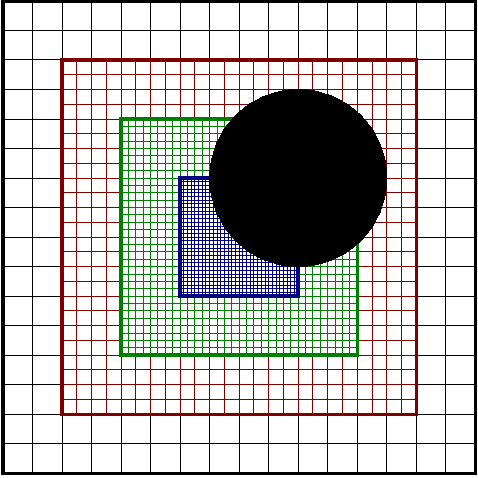
\includegraphics{./figures/amr}
%%     \caption{Adaptive mesh refinement}
%%     \label{fig:amr}
%% \end{figure}

Adaptive Mesh Refinement (AMR) grids are used by allowing overlapping grids with varying resolutions. We work with a set of grids $\Gamma^l$ that are nested hierarchically from the coarsest grid to the finest grid. Thus, we always require that a grid $\Gamma^l$ covers the overlapping region of a coarser grid $\Gamma^{l-1}$ and a finer grid $\Gamma^{l+1}$. In general, the use of AMR grids for streamer simulations is advantageous due to need for frequent regridding the solution; the use of a static mesh requires one to fully resolve the entire spatial region at the finest length scale, which leads to excessive resource requirements. Moreover, the computational overhead for remeshing a spatial region using Cartesian AMR is usually negligible (unlike Delaunay triangulation and least-squares reconstruction, for example). 

Internal boundary conditions are resolved by cutting some of the cells with a level-set function $s(\bm{x}) = 0$ which describes the boundary interface. Inside each cut-cell, the boundary is linearized so that it intersects through the cell as a line in 2D, and a plane in 3D. Control volume faces that are cut by this surface are referred to as cut-faces, and the boundary itself is referred to as an embedded boundary (EB). 

\begin{figure}[ht]
    \centering
    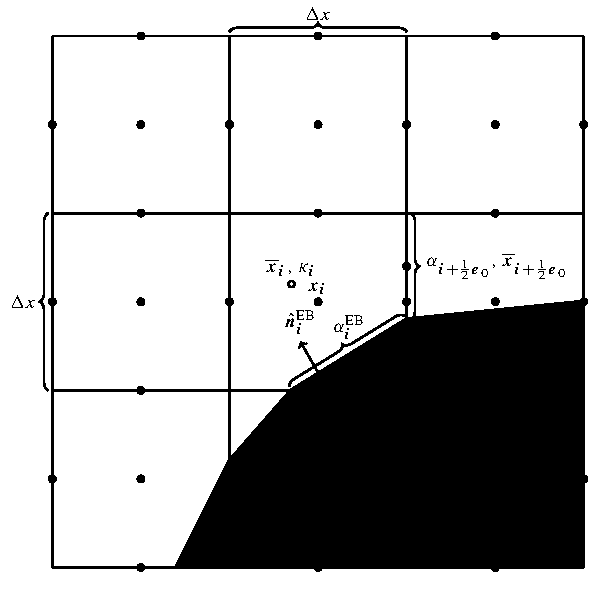
\includegraphics{./figures/spatial_discretization}
    \caption{Cut-cell discretization.}
    \label{fig:spatial_discretization}
\end{figure}

Figure~\ref{fig:spatial_discretization} shows the grid hierarchy and the cut cells in greater details. Here, a cell is identified by it's index $\bm{i}$. We will take $\bm{x}_{\bm{i}}$ to be the \emph{cell center}, and $\overline{\bm{x}}_{\bm{i}}$ to the be \emph{cell centroid}. The volume fraction is $0 \leq \kappa_{\bm{i}} \leq 1$: Cells with $\kappa_{\bm{i}} = 0$ are denoted as \emph{covered} cells and lie completely outside the computational domain; cells with volume fractions $0 < \kappa_{\bm{i}} < 1$ are called \emph{irregular} cells and lie partially inside the computational domain (see e.g. the middle cell in Fig.~\ref{fig:spatial_discretization}). Furthermore, cell faces are denoted by $f^\pm_d(\bm{i})$ where $\pm$ indicates the high ($+$) or low ($-$) face of the cell $\bm{i}$ in the coordinate direction $d$. A face center for face $f^\pm_d(\bm{i})$ is therefore located at $\bm{x}_{\bm{i} \pm \frac{1}{2}\mathbf{e}_d}$ where $\mathbf{e}_d$ is a unit vector in the $d$-direction. Face centroids are likewise denoted $\overline{\bm{x}}_{\bm{i} \pm \frac{1}{2}\mathbf{e}_d}$ and the corresponding area fractions are denoted by $\alpha_{\bm{i}\pm\frac{1}{2}\bm{e}_d}$. Finally, the EB centroid is denoted by $\overline{\bm{x}}_{\bm{i}}^{\text{EB}}$ with a corresponding area fraction $\alpha^{\text{EB}}_{\bm{i}}$ and an outward normal vector $\bm{n}_{\bm{i}}$ .

To derive the above quantities, let $V_{\bm{i}}$ denote the part of the Cartesian cell inside the computational domain, $A_{\bm{i}}^{\pm, d}$ be the un-cut part of a face $f^{\pm}_d(\bm{i})$, and $A_{\bm{i}}^{\text{EB}}$ be the part of the EB that intersects with the cell. The above quantities are given by
\begin{subequations}
  \begin{align}
    \overline{\bm{x}}_{\bm{i}} &= \frac{1}{\Delta x^{\bm{D}}}\int_{V_{\bm{i}}}\bm{x}\diff V_{\bm{i}},\\
    \overline{\bm{x}}_{\bm{i}\pm\frac{1}{2}\bm{e}_d} &= \frac{1}{\Delta x^{\bm{D}-1}}\int_{A_{\bm{i}}^{\pm, d}}\bm{x}\diff A_{\bm{i}}^{\pm, d},\\
    \overline{\bm{x}}_{\bm{i}}^{\text{EB}} &= \frac{1}{\Delta x^{\bm{D}-1}}\int_{A_{\bm{i}}^{\text{EB}}}\bm{x}\diff A_{\bm{i}}^{\text{EB}}, \\
    \kappa_{\bm{i}} &= \frac{1}{\Delta x^{\bm{D}}}\int_{V_{\bm{i}}}\diff V_{\bm{i}},\\
    \alpha_{\bm{i}\pm\frac{1}{2}\bm{e}_d} &= \frac{1}{\Delta x^{\bm{D}-1}}\int_{A_{\bm{i}}^{\pm, d}}\bm{x}\diff A_{\bm{i}}^{\pm, d},\\
    \alpha_{\bm{i}}^{\text{EB}} &= \frac{1}{\Delta x^{\bm{D}-1}}\int_{A_{\bm{i}}^{\text{EB}}}\diff A_{\bm{i}}^{\text{EB}}, \\
    \bm{n}_{\bm{i}} &= \frac{1}{\Delta x^{\bm{D}-1}}\int_{A_{\bm{i}}^{\text{EB}}}\bm{n}\diff A_{\bm{i}}^{\text{EB}}.
  \end{align}
\end{subequations}

For brevity's sake, we will from now on omit the dependency on $\bm{i}$, and re-specify this when necessary. 

\subsection{Poisson \& Eddington equations}
\label{sec:poisson}
We use the finite volume method for the Poisson equation and Eddington equations. Since the Eddington equations contain an additional diagonal term, it is sufficient to restrict our discussion to the Poisson equation.

Integrating the Poisson equation over a cell volume $V_{\bm{i}}$ yields 
\begin{equation}
  \label{eq:poisson_operator}
  \frac{1}{\kappa_{\bm{i}}\Delta x}\left[\sum_{f\in f_d^+(\bm{i})}\alpha_f\epsilon_fg_f^d - \sum_{f\in f_d^-(\bm{i)}}\alpha_f\epsilon_fg_f^d - \alpha_{\bm{i}}^{\text{EB}}\epsilon_{\bm{i}}^{\text{EB}}\left(\bm{g}^{\text{EB}}_{\bm{i}}\cdot\bm{n}_{\bm{i}}\right)\right] = \rho_{\bm{i}} + \sigma_{\bm{i}},
\end{equation}
where $g_f^d$ is the flux through the face $f$. This is discretized by using second-order approximations for the fluxes $g_f^d$ through each cell face. Note that each Cartesian face may consist of several sub-faces. For example, cells that are cut by the dielectric surface will contain two faces; one of the gas phase and one for the solid phase. This is strictly speaking not the case for faces that are cut by conducting surfaces because there is no flux passing into the volume through the part of the face that lies within the conductor. Note also that in Eq.~\eqref{eq:poisson_operator}, the embedded boundary is only the conductor surfaces. The contribution of the EB fluxes for the dielectric are contained entirely within $\sigma_{\bm{i}}$, thus avoid the need for specialized boundary condition stencils for such cells. 

For un-cut faces we discretize using
\begin{equation}
  g_f^d = \frac{1}{\Delta x}\left(\phi_{\bm{i}^+}-\phi_{\bm{i}^-}\right),
\end{equation}
where $\bm{i}^\pm$ denotes the control volumes on the high ($+$) and low ($-$) sides of the face $f$. In order to maintain a second order scheme, cut-face fluxes are interpolated to their respective centroids

\subsubsection{Multigrid solver}
The discretized Poisson equation is solved by embedding it in a geometric multigrid solver in residual-correction form. Multigrid involves iterative relaxation on progressively coarsened grids and is also compatible with AMR. On the coarsest level, the discretized system is solved directly with a biconjugate gradient stabilized method. Typically, better convergence for each cycle is achieved the further one coarsens; for domains without embedded boundaries one may coarsen up to a level where the domain only consists of two cells in one of the coordinate direction. However, for embedded boundary applications the convergence rate is usually harmed by coarsening too far because the coarsened stencils near embedded boundary may no longer be a good approximation of the finer stencils. Moreover, over-coarsening may also lead to geometrical under-resolution. We avoid both of these issues by dropping to the bottom solver before the convergence rate drops. 

\subsubsection{Boundary conditions}
For the Poisson equation we use either Dirichlet or Neumann boundary conditions on the domain edges, and Dirichlet on the conductors. Neumann boundary conditions are straightforward to implement since they specify the boundary flux directly, whereas Dirichlet is more involved. To compute Dirichlet boundary conditions we use the Johansen-Colella method by casting a ray from the EB centroid along the EB normal into the computational domain. In two dimensions, this ray will cross a coordinate line connecting two cell-centers, and the interpolated value at this point may be used to approximate the derivative $\partial_n\phi$ on the EB centroid by polynomial interpolation and differentiation. In practice, we use a second order stencil if we can, but we remark that even with a first order stencil the schme is second order due to the residual-correction form of the multigrid solver. 

%% \subsection{Convection-Diffusion-Reaction equations}
%% For the mass transport equation we apply the method of Godunov with van Leer limiting. For definiteness, it is sufficient to discuss the advective part of the equation in the form
%% \begin{equation}
%%   \frac{\partial n}{\partial t} + \nabla\cdot(\bm{v}n) = S - \nabla\cdot\left(D\nabla n\right).
%% \end{equation}

%% \subsubsection{Hybrid divergence}


%% \subsection{Eddington equations}
%% The Eddington equations 

%% \subsection{Temporal discretization}
 
\section{Numerical examples}
\label{sec:examples}

\section{Concluding remarks}
\label{sec:remarks}
Finally, we wish to provide a few concluding remarks regarding streamer simulations. In our opion, we anticipate that there is much to be gained by community-driven improvements of the radiative transfer in streamers. Firstly, let us remark that the stationary simplification that is frequently used for radiative transport codes in streamer simulations is only weakly applicable, and certainly not valid for atmospheric discharge which take place on length scales of hundreds or even thousands of meters. In addition, all diffusion-based RTE methods neglect even qualitative features such as geometrical shading, and we broadly believe that improved radiative transport codes should be implemented into existing streamer code frameworks. Since direct integration of the RTE is unpractical in three dimensions, the obvious candiates for RTE simplification are the discrete ordinates method (DOM) and moment-based RTE. Discrete ordinates essentially solve the RTE by sampling the propagation angles $\bm{\Omega}$ on a finite angular grid and can be implemented straightforwardly using existing CDR framework since the angularly discretized RTE is essentially, a set of advection equations. Unfortunately, the DOM is likely to become a computational bottleneck in both CPU and memory since the numerical sampling of angular space must be large in order avoid numerical artifacts. We therefore suggest that the community investigates moment-based RTE with improved closure relations are. In this case, the RTE reduces to three (four) hyperbolic conservation equations in 2D (3D) for each frequency group. For causal reasons those equations should be solved using higher order methods, such as those of Godunov. 


%\section{Conclusions}

%\section*{Acknowledgements}
%This work was financially supported by the Norwegian Research Council, ABB Skien, and ABB CRC. The author expresses his gratitude to D. T. Graves for help regarding multigrid and Godunov methods, and S. Pancheshnyi for fruitful discussions regarding plasma kinetics in air. 

\end{document}
